Para a construção estrutural do robô utilizamos materiais fornecidos gentilmente pelo Professor Douglas Macharet (UFMG/DCC) e também materiais adquiridos pelos alunos integrantes deste trabalho. Nas subseções 2.1 e 2.2 descrevemos os materiais e métodos utilizados para o desenvolvimento do robô

\subsection{Materiais}

Para arquitetar a estrutura do robô utilizamos peças de Lego (Figura \ref{lego1}). Um kit de peças de lego como esse têm como uma de suas finalidades a construção de robôs, oferecem uma grande quantidade de peças que facilitam o projeto e tornam mais prática a sua execução.

\begin{figure}[!htb]
	\centering
	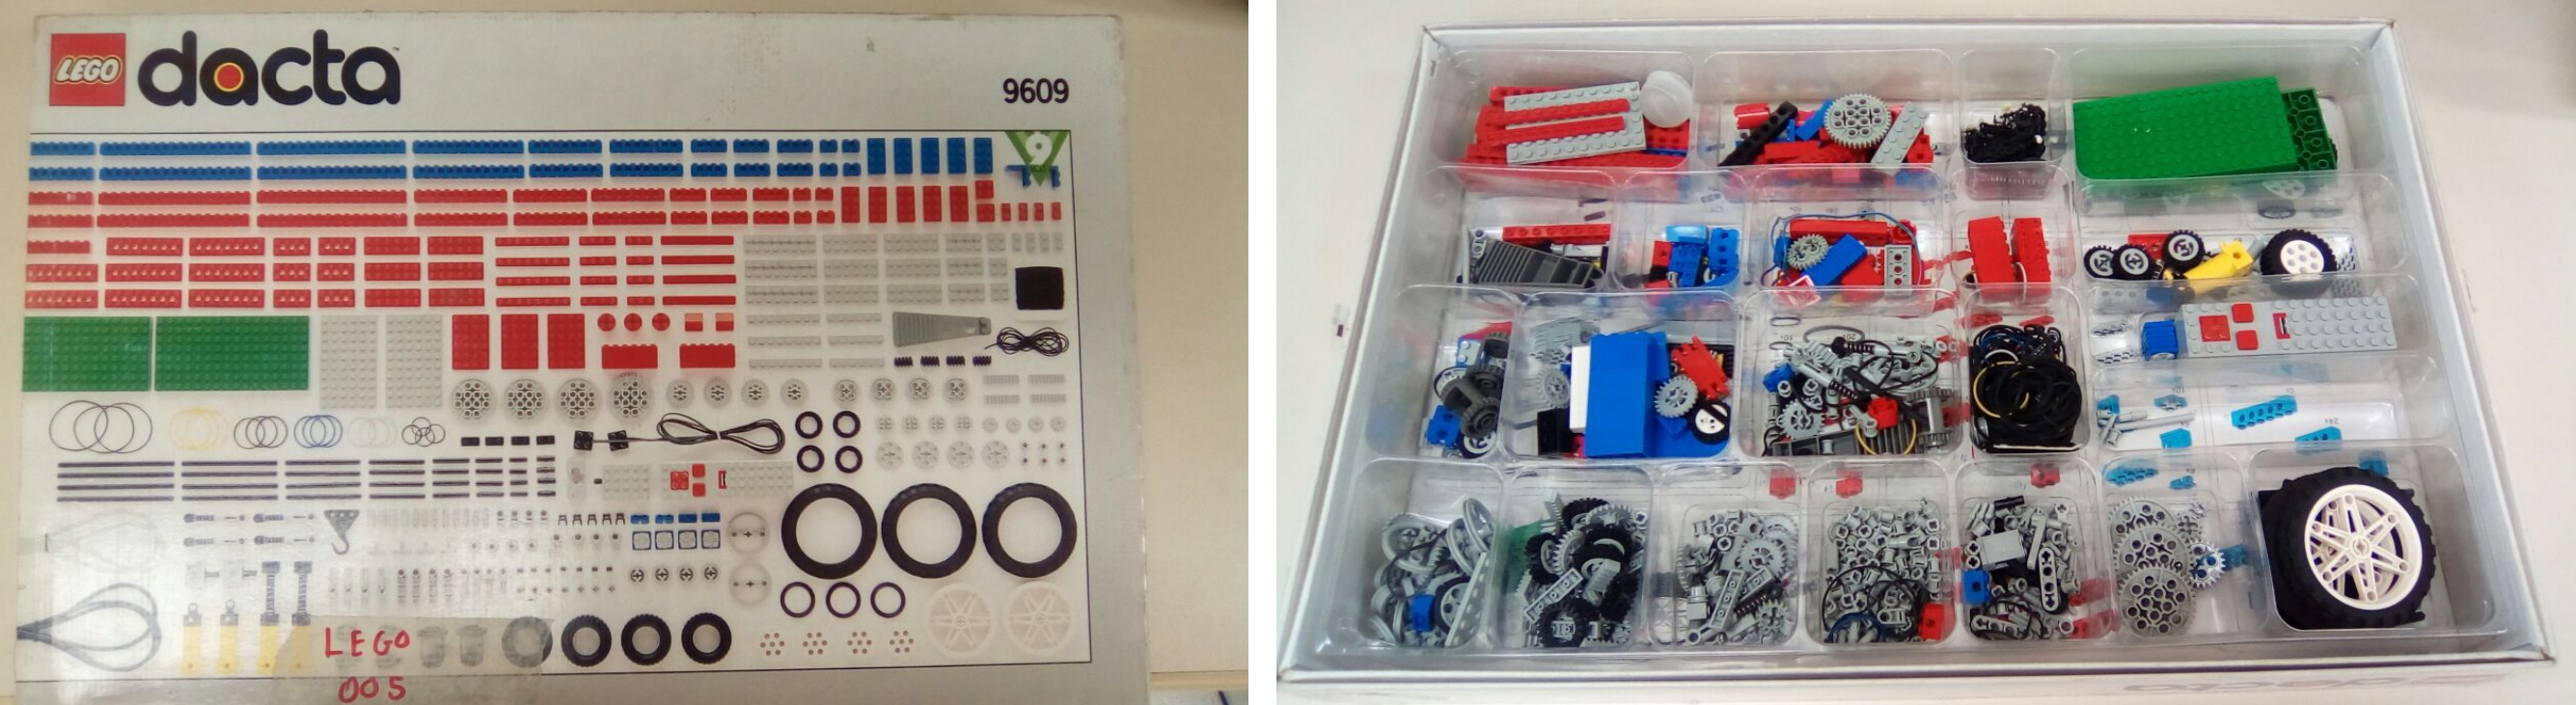
\includegraphics[width=12.5cm]{images/lego1.png}
	\caption{Kit de Lego.}
	\label{lego1}
\end{figure}

Para permitir que o robô realize as tarefas é necessário uma plataforma que permita integrar os sensores (Figuras \ref{sensores1}, \ref{sensores2}, \ref{sensores3} e \ref{sensores4}) que precisamos para a execução das mesmas. A plataforma escolhida foi o Arduino (Figura \ref*{arduino}), uma plataforma eletrônica de código aberto.


\begin{figure}[!htb]
	\centering
	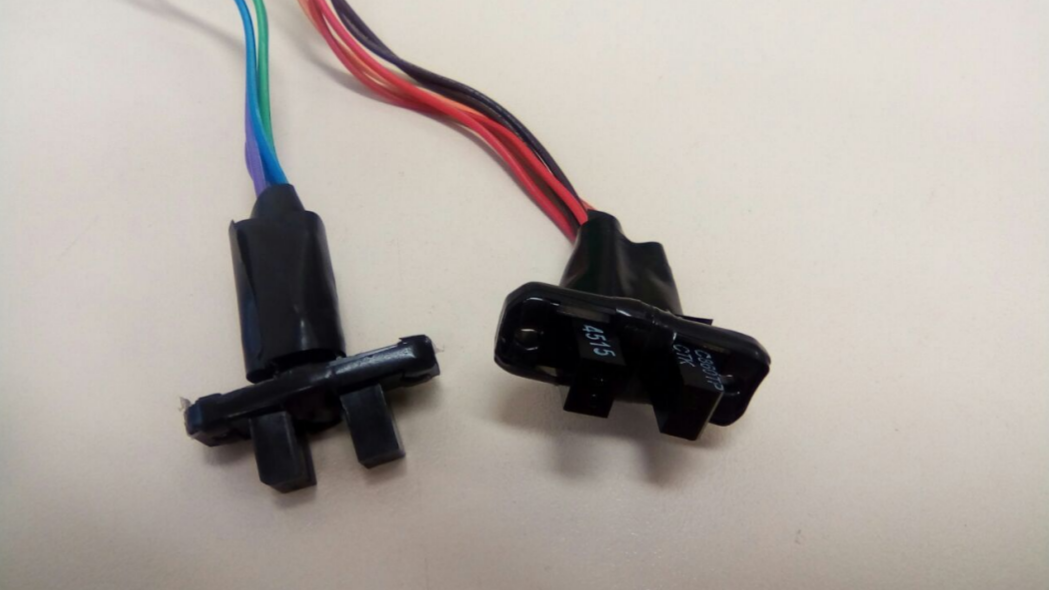
\includegraphics[width=9cm]{images/sensores1.png}
	\caption{Sensores Break Beam}
	\label{sensores1}
\end{figure}


\begin{figure}[!htb]
	\centering
	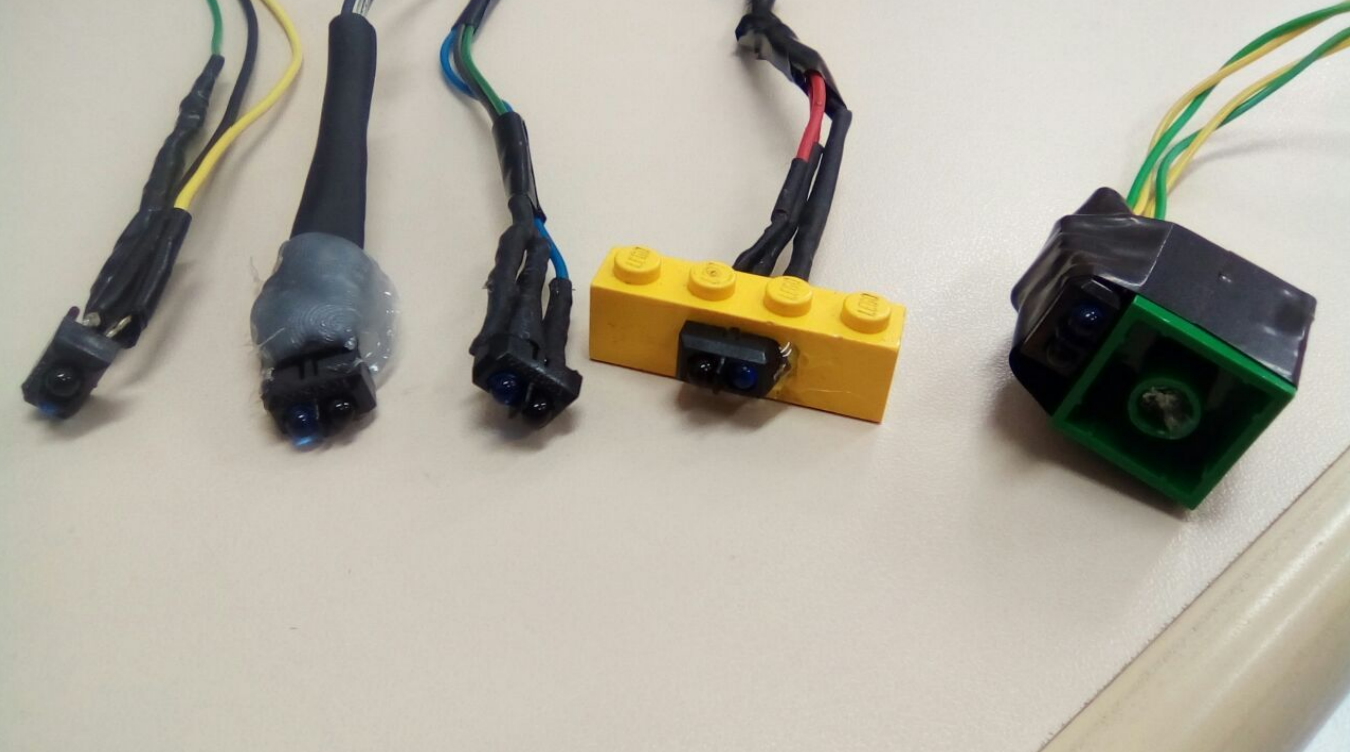
\includegraphics[width=9cm]{images/sensores2.png}
	\caption{Sensores Óptico Reflexivos}
	\label{sensores2}
\end{figure}

\begin{figure}[!htb]
	\centering
	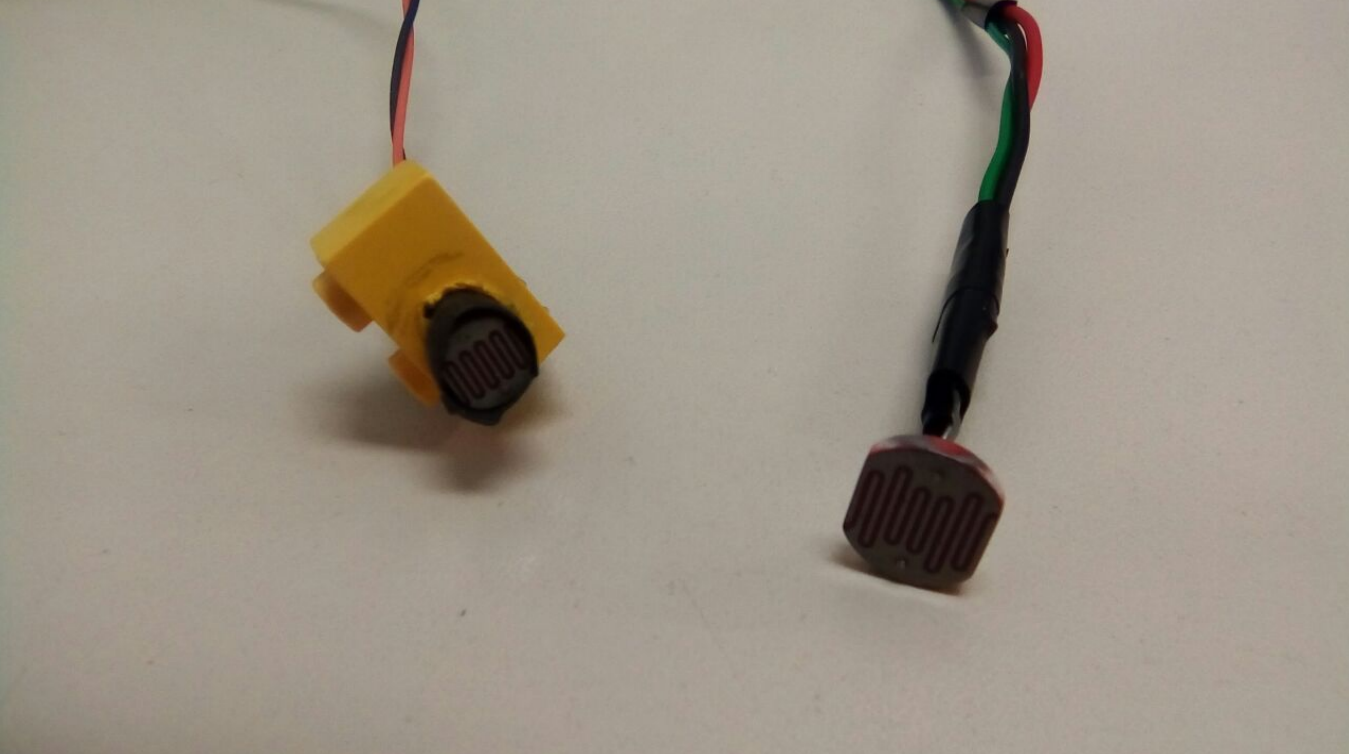
\includegraphics[width=9cm]{images/sensores3.png}
	\caption{Sensores LDR}
	\label{sensores3}
\end{figure}

\begin{figure}[!htb]
	\centering
	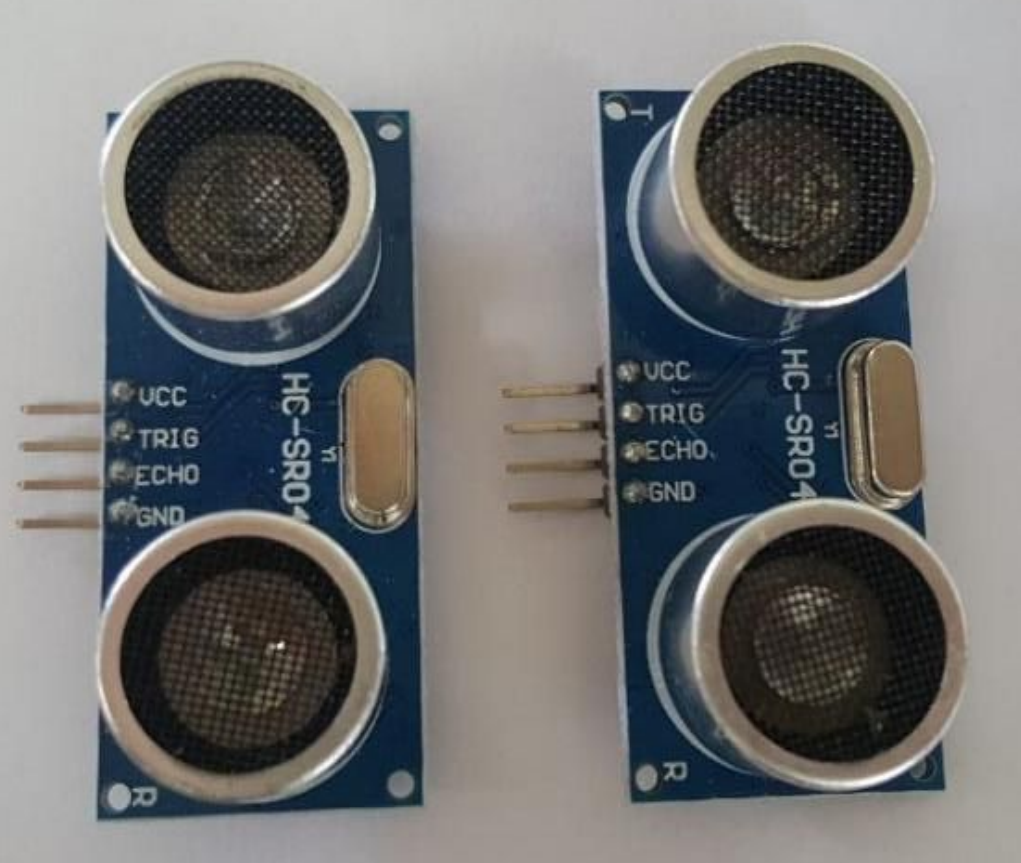
\includegraphics[width=7cm]{images/sensores4.png}
	\caption{Sensores Ultrassônicos}
	\label{sensores4}
\end{figure}

\begin{figure}[!htb]
	\centering
	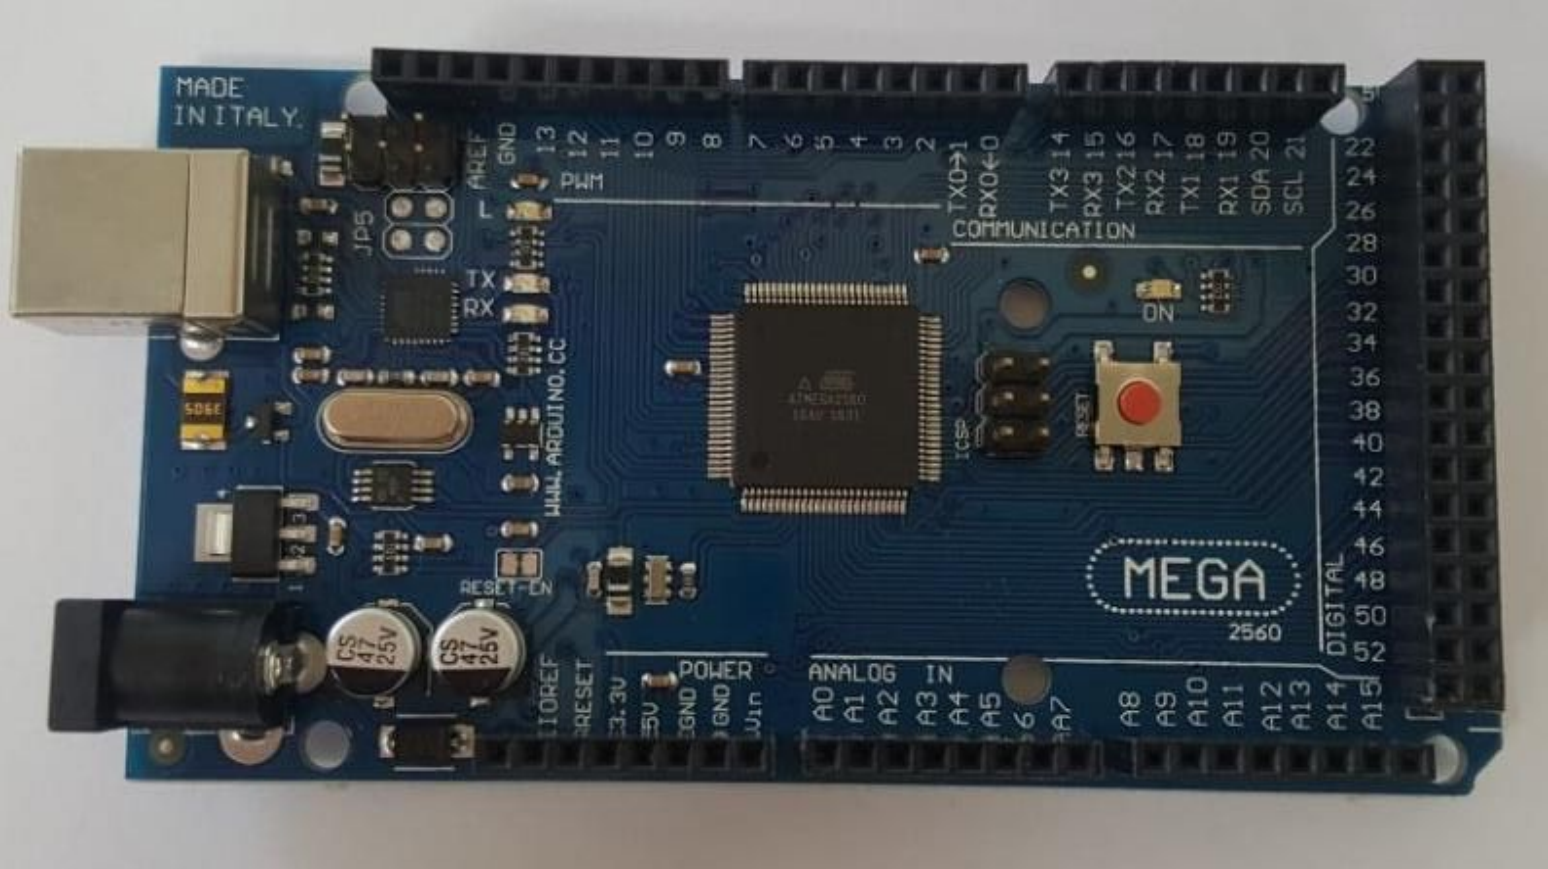
\includegraphics[width=8cm]{images/arduino.png}
	\caption{Plataforma Arduino}
	\label{arduino}
\end{figure}

\newpage

Para realizar o controle de motores com nossa placa Arduino, adquirimos um Motor Shield - Driver Ponte H (Figura \ref{shield}).

\begin{figure}[!htb]
	\centering
	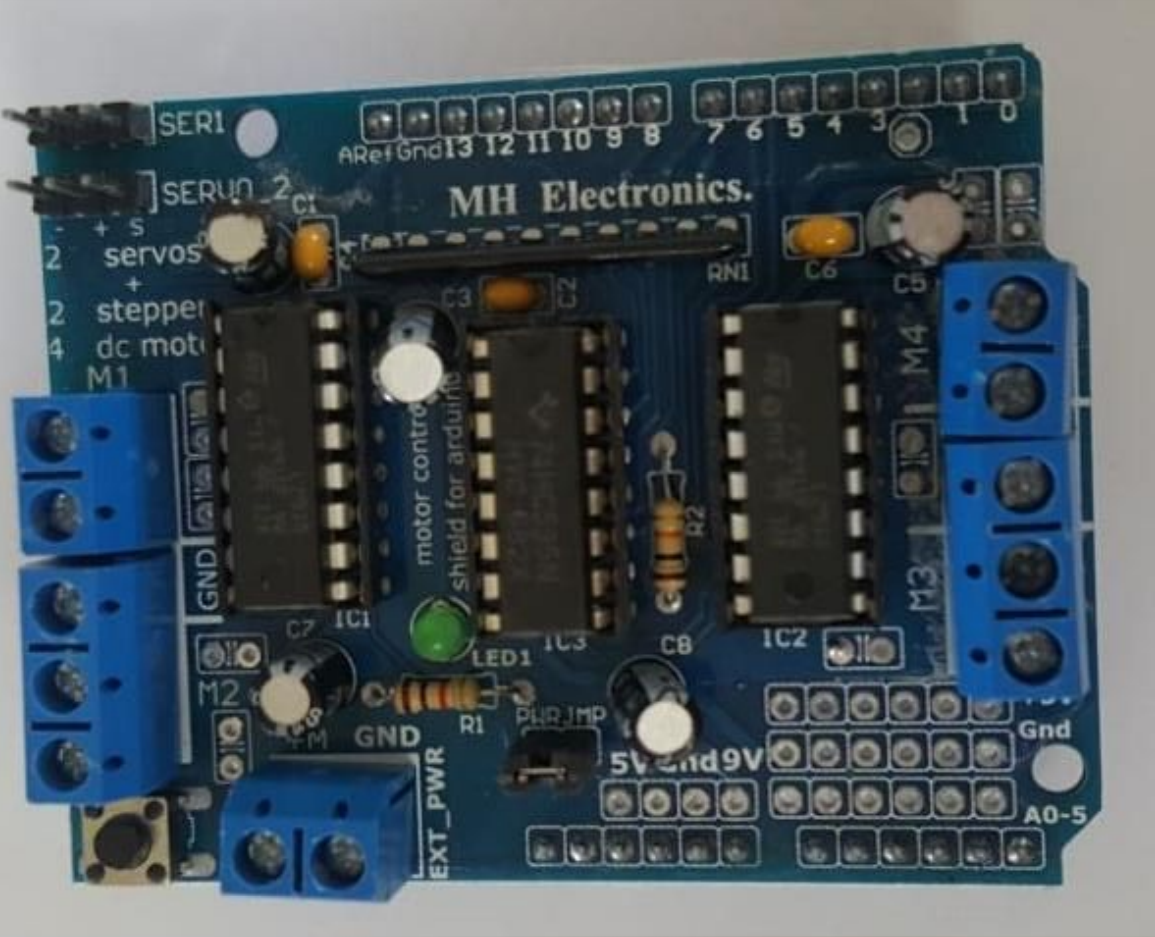
\includegraphics[width=8cm]{images/shield.png}
	\caption{Motor Shield - Driver Ponte H}
	\label{shield}
\end{figure}

\newpage

Após a montagem da estrutura e alocação dos sensores o robô ficou como mostrado na Figura \ref{robo}. 

\begin{figure}[!htb]
	\centering
	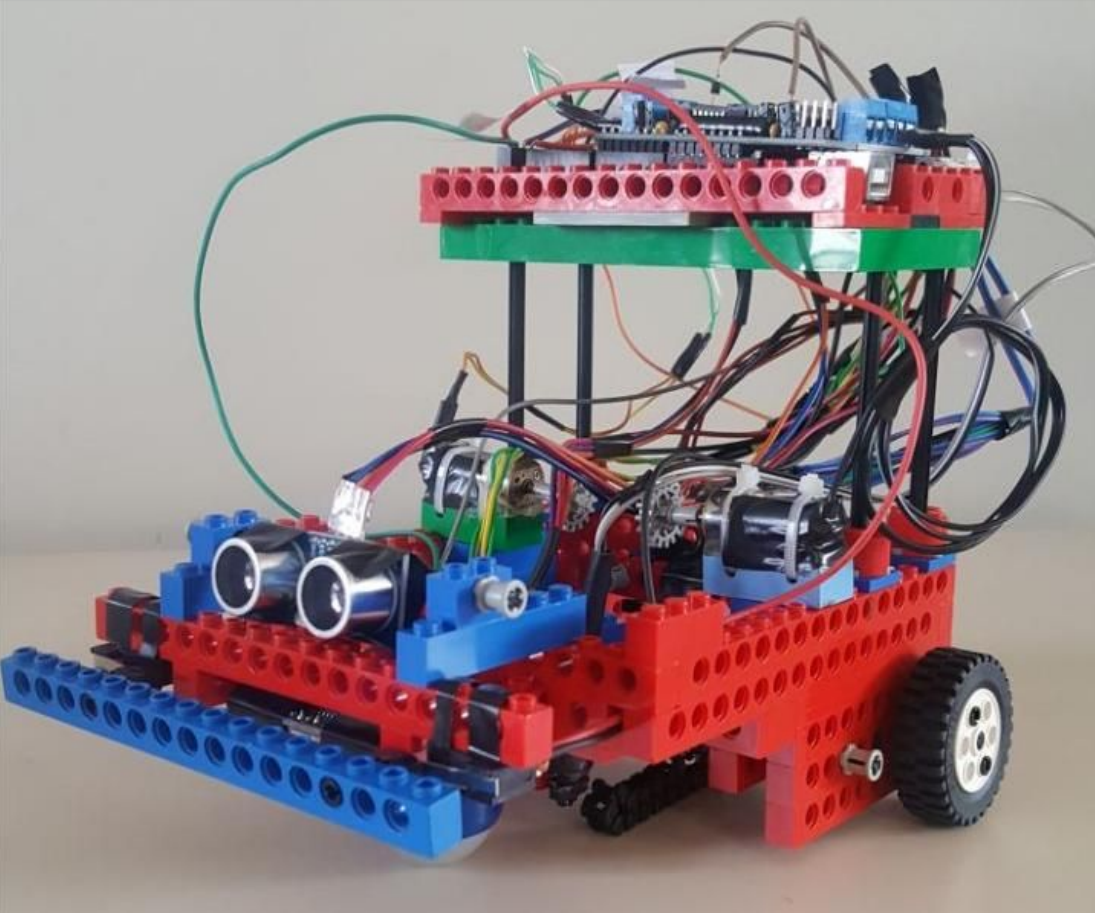
\includegraphics[width=10cm]{images/robo.png}
	\caption{Robô com estrutura finalizada.}
	\label{robo}
\end{figure}


\subsection{Métodos}

Para a montagem da estrutura do robô utilizamos o kit de Legos de forma a deixar o Arduíno, o Motor Shield e os sensores bem adaptados. Para a montagem e soldagem dos sensores nós utilizamos tutoriais ilustrados que podem ser facilmente obtidos na internet. Todos os sensores foram testados e apresentaram boa performance.

// Melhorar.